\chapter{Introduction}

\label{introduction}

Some parts of this section is derived from the definitions provided here \url{https://conp.ca/about-the-conp/}
%what is open science?
Traditionally, the scientific research were conducted in the research or academic institutions and were kept there. That was Closed Science, where after the findings were published, the data were often inaccessible to others due to privacy issues and ownership of the resources. This made data difficult to find and access and therefore, made further research on that subject slower. For such reasons, Open Science emerged with the purpose of preparing and releasing the data to the whole scientific community worldwide, so they can collaborate in research and discovery which leads to faster growth of findings.

Open Science is referred as an umbrella term covering open dissemination of data, manuscripts, software, materials, methodologies and other outputs which scientists produce in their research. Open Science also aims to make the scientific process more transparent and accessible. Open Science research allows others to collaborate and contribute to the study using freely available research data and all the resources in the research process, which facilitates the reuse, redistribution and reproduction of the research outcome and its underlying data and methods~\cite{bartling2014opening}.

%why open science is important?
In Open science it is highly important to share the resources correctly and make the research findings reproducible sine due to malpractice in many of current methods for sharing and capturing data, "approximately 50\% of all research data and experiments is considered not reproducible, and the vast majority (likely over 80\%) of data never makes it to a trusted and sustainable repository.”~\cite{ayris2016realising}

Moreover, Open Science is increasingly important in current science world, beneficial for scientists, patients, and the public and has emerged as a framework to improve the quality of scientific analysis. There are several reasons why Open Science is important, the findings and output of publicly funded scientific research would be more available and accessible, therefore the scientific works would be more transparent and reproducible. Also, the public implication would be possible in conducting the research and might impact on the results. Also open peer-review would be possible which encourages wider and more transparent review processes by extending knowledge exchange between researchers~\cite{wolfram2020open,ross2019guidelines}. 


% how open science is defined? any other definition that FAIR?
There are different definitions for the concerns and principles required to follow in Open Science. As mentioned above, Open Science encompasses a variety of areas including open access to publications, open research data, open source software/tools, open workflows, open educational resources, and alternative methods for research evaluation including open peer-review\cite{pontika2015fostering}. To implement these practices, there is a set of five broad concerns as "schools of thought" to be considered which is defined by Fecher \& Friesike in 2014~\cite{fecher2014open}. 

These concerns are represented in Figure~\ref{fig:5school}: 'Democratic school' which believes the scholarly knowledge (including publications and data) should be available freely for all. Second one is 'Pragmatic school' which aims at making scholarly methods transparent and concerns with efficient knowledge creation through collaboration and critique. Third is 'Infrastructure school' mentioning "efficient research requires readily available platforms, tools and services for dissemination and collaboration"\href{https://open-science-training-handbook.gitbook.io/book/open-science-basics/open-concepts-and-principles}{from here}. The forth is 'Public school' claiming that the public should be able to collaborate in research and the scholarship should be more readily understandable for all through less formal communicative methods. The last one is 'Measurement school' that believes it is required to define alternative metrics to track and measure the impact of scholarship.

\begin{figure*}[ht]
  \centering
  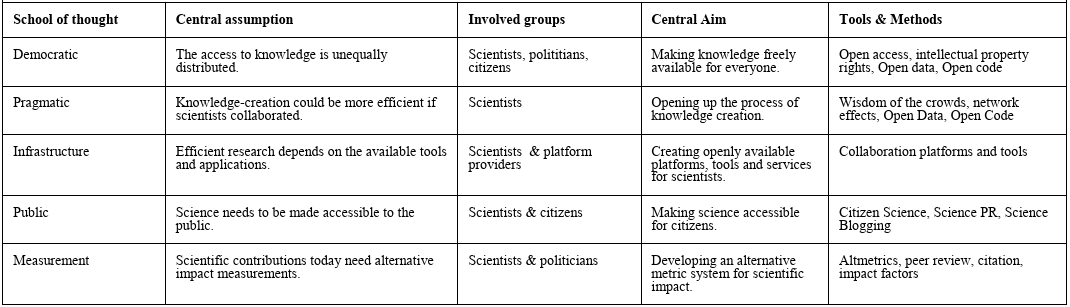
\includegraphics[width=\textwidth]{figures/5schools.png}
  \caption{Five Open Science Schools of Thought. Figure is captured from~\cite{fecher2014open} }
  \label{fig:5schools}
\end{figure*} 


The next widely referred definition for principles of Open Science is defined by Wilkinson in 2016 as FAIR principles~\cite{wilkinson2016fair} which claims that the research should be Findable, Accessible, Interoperable, and Reusable for all users. Many of the currently available platforms for sharing resources are trying to guarantee the FAIR principles. Each one the principles in FAIR are explained in the background section.  

%open science in nouroscuience meaning
Open Science is affects on almost all areas in scientific research studies, particularly neuroscience which is the study of the nervous system. Open science practices can help to address many challenges in neuroscience. For instance, the answer of many key questions in neuroscience can be found when the research findings and outputs are openly shared. In this case, people also can collaborate and help in discovery of innovative solutions for the treatment of brain-related illnesses. 

%data sharing in neuroscience
The resources to be shared in neuroscience include the datasets consisting of raw data, pre-processed data or the result of analysis applied to raw or pre-processed data which should be shared on data sharing platforms. The data sharing platforms in neuroscience and other health related areas are mostly following the principles defined by National Institutes of Health (NIH)available~\href{https://grants.nih.gov/grants/policy/data_sharing/data_sharing_guidance.htm}{here}. According to these principles "Data should be made as widely and freely available as possible while safeguarding the privacy of participants, and protecting confidential and proprietary data". \href{https://loris.ca/index.html}{LORIS} is and open-source framework for storing, processing and sharing behavioural, clinical, neuroimaging and genetic data. Also \href{https://www.braincode.ca/}{Brain-CODE} is "A Secure Neuroinformatics Platform for Management, Federation, Sharing and Analysis of Multi-Dimensional Neuroscience Data"~\cite{vaccarino2018brain}.


% tools are required to process the data, tool sharing in neuroscience 

The data itself is not enough in neuroscience research studies, there are a set of neuroimaging tools and pipelines for processing the data that should be shared as well. Therefore, to guarantee open science principles in neuroscience, it is required to use platforms for sharing neuroscience datasets and neuroimaging tools and pipelines as well as the possible outcome of conducted analysis. There are many neuroscience data and tool sharing platforms such as \href{https://canadianbrain.ca/mission-vision/}{Canadian Brain Research Strategy (CBRS)}, \href{https://www.nitrc.org/}{NeuroImaging Tools \& Resources Collaboratory (NITRC)}, \href{https://openneuro.org/}{OpenNeuro} and \href{https://conp.ca/}{Canadian Open Neuroscience Platfrom}. Three of these platforms are explained in this thesis NITRC and OpenNeuro in chapter two and CONP in chapter three.



%the problem we focused on?
Although there are many platforms for data and tool sharing in neuroscience, there is still lacking of a system to help users  bridging the datasets and tools together when they are going to conduct and analysis. Using current platforms, in the best scenario, the users are able to see the outcome of analysis applied on data. However, providing a list of possible tools/pipelines for a data/dataset will facilitate the process of analysis for the user and prevents the confusing and time-consuming process of selecting an appropriate tool/pipeline for the candidate data/dataset, the same scenario would be helpful when the user needs to select data/dataset to execute a candidate tool/pipeline.

The goal of this thesis is to investigate the feasibility of implementing a recommender system to recommend appropriate tools/pipelines and data/datasets given the other based on the available records from previous executions. Consistently with our motivating use case, we focused on the available neuroscience tools/pipelines and data/datasets(from now on 'pipeline' and 'dataset') in Canadian Open Neuroscience Platform(CONP) available at \url{https://portal.conp.ca/index}. The pipelines in CONP are described in Boutiques~\cite{glatard2018boutiques} which is software library for sharing tools according to the FAIR principles. CONP has distributed datasets in  neuroimaging, transcriptomics, genomics, and other related data modalities. More details about the CONP and its available pipelines and dataset is provided in chapter three.



Recommender systems are widely used and increasingly being successful in satisfying the users by suggesting the items they might like and helping them selecting the better choices faster. There have been many successful works on recommender systems such as Netflix~\cite{bennett2007netflix} for movie recommender and Amazon~\cite{7927889} as product recommender. There are two main strategies for recommender systems, Collaborative Filtering~\cite{rajaraman2011mining} which propose recommendations based on the user-item interactions, recommending an item to a user if it is liked by similar users, the other approach is Content-based Filtering~\cite{pazzani2007content} which recommends a user the similar items to their previous choices.  

For our project we focused on collaborative filtering to  recommend neuroimaging data/datasets and tools/pipelines given the other. In this case we have a database of the previously executed pipeline-dataset pairs and apply a collaborative filtering model on that to get the recommended items. We did not select content-based approach for the recommender system since in this case there should be accurate and comprehensive descriptions for all datasets and pipelines while these descriptions are manually written by some colleagues in CONP and are not reliable and consistent.   

 

% what will be in this thesis?

This thesis is organized as follows, in chapter two we explain the details about the required components and background knowledge, chapter three explains the Canadian Open Neuroscience Platform (CONP), chapter four is the whole approach for this project and is submitted as a conference paper to \href{https://supercomputing.org/}{The International Conference for High Performance Computing, Networking, Storage, and Analysis}. Finally chapter five expand the conclusions and explains more about the possible future works on this project.


